% Preamble ==================================================================
\documentclass[11pt]{article}
\usepackage{geometry}
\geometry{verbose,tmargin=2.5cm,bottom= 1.5cm,lmargin=2.5cm,rmargin=2.5cm}
\usepackage{float}
\usepackage{graphicx}
\usepackage{amsmath}
\usepackage{amssymb}
\usepackage{enumitem}
\usepackage{mathtools}

\usepackage{amsthm} % theorem
\usepackage{listings} % code snippets
\usepackage{fancyvrb} %verbatim
\lstset{frame=l,
  language=Python,
  basicstyle={\small\ttfamily},
  numbers=none,
  numberstyle=\tiny\color{black},
  keywordstyle=\color{black},
  commentstyle=\color{blue},
  stringstyle=\color{mauve},
}

\numberwithin{equation}{section}

\usepackage{titlesec,dsfont}

%Format section heading style
\usepackage{sectsty}
\sectionfont{\sffamily\bfseries\large}
\subsectionfont{\sffamily\normalsize\slshape}
\subsubsectionfont{\sffamily\small\itshape}
\paragraphfont{\sffamily\small\textbf}


%Put period after section number
\makeatletter
\def\@seccntformat#1{\csname the#1\endcsname.\quad}
\makeatother

%Bibliography
\usepackage[round]{natbib}
\bibliographystyle{genetics}

%Format captions
\usepackage[ labelsep=period, justification=raggedright, margin=10pt,font={small},labelfont={small,normal,bf,sf}]{caption}

\setlength{\parskip}{0ex} %No space between paragraphs.

\renewcommand{\familydefault}{\sfdefault}

\newcommand\indep{\protect\mathpalette{\protect\independenT}{\perp}}
\newcommand{\nindep}{\not\!\perp\!\!\!\perp}
\def\independenT#1#2{\mathrel{\rlap{$#1#2$}\mkern2mu{#1#2}}}

%PUT ME LAST--------------------------------------------------
\usepackage[colorlinks=true
,urlcolor=blue
,anchorcolor=blue
,citecolor=blue
,filecolor=blue
,linkcolor=black
,menucolor=blue
,linktocpage=true
,pdfproducer=medialab
,pdfa=true
]{hyperref}

\makeatother %Put this last of all


\newcommand{\defeq}{\coloneqq}
\newcommand{\overbar}[1]{\mkern 1.5mu\overline{\mkern-1.5mu#1\mkern-1.5mu}\mkern 1.5mu}

% Make theorems bold
\makeatletter
\def\th@plain{%
  \thm@notefont{}% same as heading font
  \itshape % body font
}
\def\th@definition{%
  \thm@notefont{}% same as heading font
  \normalfont % body font
}
\makeatother

\newtheorem{thm}{Theorem}[section]
\newtheorem{defn}{Definition}[section]
\newtheorem{cor}{Corollary}[section]
\newtheorem{prop}{Property}[section]
\newtheorem{rle}{Rule}[section]
\newtheorem{lma}{Lemma}[section]

%Preamble end--------------------------------------------------


\begin{document}

\begin{flushleft}
\textbf{\Large Sequence models}
\end{flushleft}

\begin{flushleft}
Author: Juvid Aryaman

Last compiled: \today
\end{flushleft}

\noindent This document contains my personal notes on sequence models.


\section{Embeddings}
Embeddings are tensors. You interact with that tensor by indexing into it. It is often used to store encodings of collections of words. For example:
\begin{lstlisting}
>>> nn.Embedding(vocab_sz, n_hidden)
\end{lstlisting}	
creates a set of \verb#vocab_sz# tensors, each of size \verb#n_hidden#. 

A common thing to do is to something like:
\begin{lstlisting}
>>> embedding = nn.Embedding(10, 3)
>>> input = torch.LongTensor([[1,2,4,5],[4,3,2,9]])
>>> embedding(input)

tensor([[[-0.0251, -1.6902,  0.7172],
         [-0.6431,  0.0748,  0.6969],
         [ 1.4970,  1.3448, -0.9685],
         [-0.3677, -2.7265, -0.1685]],

        [[ 1.4970,  1.3448, -0.9685],
         [ 0.4362, -0.4004,  0.9400],
         [-0.6431,  0.0748,  0.6969],
         [ 0.9124, -2.3616,  1.1151]]])
\end{lstlisting}
so you can see that the input is \verb#[sentence1, sentence2]#, where sentence 1 consists of words \verb#[1,2,4,5]#. As an output, we get the corresponding 3-vectors for each word. So the output is: 
\begin{lstlisting}
[[[embedding_word_1,   # length 3 vector
   embedding_word_2, 
   embedding_word_4, 
   embedding_word_5],
  
  [embedding_word_4, 
   embedding_word_3, 
   embedding_word_2, 
   embedding_word_9]
]]
\end{lstlisting}

\section{Linear layer}
Applies a linear transformation to the incoming data: $y = xA^T + b$
\begin{lstlisting}
>>> m = nn.Linear(20, 30)
>>> input = torch.randn(128, 20)
>>> output = m(input)
>>> print(output.size())
torch.Size([128, 30])
\end{lstlisting}


\section{Recurrent neural network}
Torch, by default, applies a multi-layer Elman RNN. This is defined as applying the following function to each element of the input sequence
\begin{align}
h_t  &= \sigma_h(W_h x_t + U_h h_{t-1} + b_h)\\
y_t  &= \sigma_y(W_y h_t + b_y)
\end{align}
where $x_t$ is an input vector, $h_t$ is a hidden layer vector, $y_t$ is an output vector, $W, U, b$ are parameter matrices and vector, $\sigma_h, \sigma_y$ are activation functions. Note that we don't actually retain the hidden state between lines -- we throw it away after every complete training example (a line). We will typically initialize the hidden state to be $h_{t=0}=0$. Within a particular training instance, on a particular line, we may have different maximum values of $t=T$. 

For example, in word classification, where we construct a character-level RNN, in each training loop we will
\begin{enumerate}[noitemsep]
\item Get an input and target tensor
\item Create a zeroed initial hidden state
\item Read each letter in and:
\begin{itemize}[noitemsep]
\item Keep hidden state for next letter
\item Feed the previous hidden state $h_{t-1}$ in with the current input $x_t$
\end{itemize}
\item Compare output at the end of the RNN loop to the target
\item Back-propagate
\end{enumerate}
Then return the output and loss.

\begin{figure}
\begin{center}
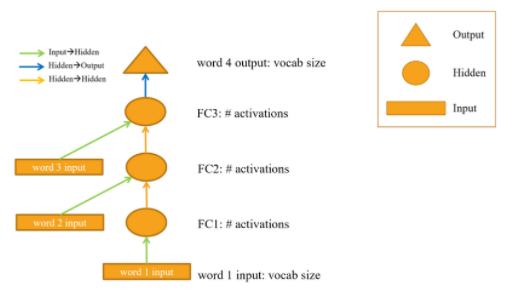
\includegraphics[width=0.8\columnwidth]{figures/rnn.png}  
\end{center}
\caption{Graphical representation of RNN
}
\label{fig:rnn}
\end{figure}

\cite{bahdanau14}


\newpage
\bibliography{seq.bib} 

\end{document}